\section{Engine - Systeme}
\subsection{Math System}

Das Math-System ist für sämtliche mathematischen Berechnungen zuständig. Dazu gehören sehr einfache Rechnungen wie Umwandlung von Grad in Bogenmaß, aber auch komplexere Rechnungen wie zum Beispiel Matrix-Rechnungen. 
Dazu beinhaltet das System mehrere Hilfsklassen, welche in anderen Systemen verwendet werden können. Die Hauptaufgabe ist die Umsetzung der linearen Algebra. 

Um den dreidimensionalen Raum des Spiels darzustellen werden in der FM3D-Engine Vektoren verwendet. Deswegen arbeitet das Math-System hauptsächlich mit Vektoren.
%removed by max
%werden auch die meisten Brechungen mit Vektoren ausgeführt.

Es gibt für Vektoren mit zwei, drei und vier Dimensionen jeweils eine \textit{Template}-Klasse. So kann man in der FM3D-Engine Vektoren mit unterschiedlichen Datentypen für einen Skalar verwenden. 
Diese \textit{Vektor}-Klassen beinhalten Methoden für mathematischen Operatoren, die auf Vektoren anwendbar. Zudem verwendet sie überladene Operatoren, um das zugreifen im Code zu erleichtern. 
Dazu gehören: 
\begin{itemize}
	\item Addition
	\item Subtraktion
	\item Multiplikation
	\item Division
	\item Bildung des Kreuz- und Skalar-Produktes
\end{itemize}

Außerdem ist es möglich die Länge des Vektors zu berechnen und normalisieren.
Es gibt für die grundlegenden Datentypen einen vordefinierten Typ, damit nicht immer ein Vektor mit Template-Parameter ausgeschrieben werden muss. 

Dieser ist folgendermaßen aufgebaut:
$$"`Vector"' + Dimension + Abkürzung des Datentyps$$
Ein dreidimensionaler Vektor mit dem Skalar-Datentyp \textit{float} wäre zum Beispiel: 
$$Vector3f$$

Zu linearer Algebra gehört selbstverständlich auch die Möglichkeit Matrizen zu transformieren.
%Removed by max
%mit Matrizen Transformationen darzustellen. 
Dafür enthält das Math-System die Matrix4f Klasse. Diese repräsentiert eine $4x4$ Matrix mit dem Skalar-Datentyp Float. Sie besitzt die Möglichkeit mit anderen Matrizen, vierdimensionalen und dreidimensionalen Vektoren, multipliziert zu werden. Sie kann auch mit anderen Matrizen addiert, sowie invertiert und transponiert werden. Außerdem enthält die Matrix4f-Klasse einige statische Methoden, um bestimmte Matrizen zu erstellen. Dazu gehören Transformations-, Rotations-, Skalierungs- und Projektionsmatrizen.

\subsection{File System}
Um Dateien verschiedener Formate in der FM3D-Engine verwenden zu können, wird die Klasse \textit{ExternFileManager} verwendet.
Die \textit{ExternFileManager} Klasse besitzt Methoden um Schriftarten, Bilder und Modelle zu laden. Der Methode \textit{ReadFontFile} um die Schriftarten zu laden übergibt man eine Referenz zu dem Namen der Datei. Zudem gibt man die Größe und die Skalierung der Schriftart an. Um die Textur auch in einem RenderSystem dar zu stellen, benötigt die Methode auch eine Referenz zu einem existierenden Objekt der \textit{RenderSystem}-Klasse. Die Methode benötigt zudem eine doppelte Referenz zu einem bereits erstelltes Objekt der Klasse \textit{Font}. 
Die Methode \textit{ReadTextureFile} gibt eine Referenz zu einem Objekt der Klasse Textur zurück. Als Übergabeparameter benötigt diese Methode zunächst das RenderSystem in dem die Textur gerendert werden soll. Außerdem benötigt diese Methode noch  die Enumerationen vom Typen \textit{FilterMode}, \textit{WrapMode} und \textit{MipMapMode}, welche in der Klasse \textit{Textur} stehen. Alle dieser Enumerationen besitzen bereits in dieser Methode einen Standardwert und müssen nicht explizit angegeben. Zur Erläuterung dieser Enumerationen siehe den \cref{Textureclass}. 
Die Methode \textit{ReadModelFile} benötigt als Übergabeparameter den Dateinamen, das RenderSystem in dem das Model geladen werden soll. Ein boolescher Übergabeparameter gibt an, ob \textit{Instancing} verwendet werden soll. Der darauffolgende  boolescher Wert gibt an, ob eine Animation in dem Model verwendet werden soll. Eine vierstellige Matrix \textit{Matrix4f} gibt die Skalierung des Models an.
Zur Initialisierung wird die Methode \textit{Initialize} verwendet.

\subsection{Graphic System}

\subsubsection{Fenster}
Jedes GUI benötigt ein \textit{Fenster}, in dem die Grafiken angezeigt werden können. Dafür existiert die Klasse \textit{Win32Window}, die von der Klasse Windows erbt, welche die Grundstruktur und Grundinformationen für ein Fenster besitzt. 
Um ein Fenster zu starten verwendet man die Methode \textit{Start}, welcher man die Größe Breite und Höhe des Fensters, den Fenstertitel übergibt. Das Fenster kann mit der Methode \textit{Close} geschlossen werden.
Aus der Klasse Windows werden \textit{Get-} und \textit{Set-}Methoden für die Größe und Position des Fensters auf dem Bildschirm und private Attribute die diese Werte angeben geerbt.
Zudem besitzt die Klasse \textit{Window} statische Methoden um ein Fenster zu erstellen, die Position eines Fensters zu bestimmen, eine Konsole zu starten und die Position dieser zu bestimmen.

\subsubsection{RenderSystem}
Um in diesem Fenster nun zu rendern benötigt man ein Objekt der Klasse RenderSystem. Das RenderSystem kontrolliert das Rendering der FM3D-Engine in der Anwendung. Diese Klasse besitzt eine Initialisierungsmethode, welcher man die Werte 

\subsubsection{Font-Klasse}
\label{Fontclass}
Objekte der Font-Klasse repräsentieren Schriftarten, welche man im Programm rendern kann.

\subsubsection{Texture-Klasse}
\label{Textureclass}
Die Klasse besitzt die Enumerationen \textit{FilterMode}, \textit{WrapMode} und \textit{MipMapMode}. In \textit{FilterMode} gibt verschiedene Filtermodi an, in denen die Textur gerendert wird.
Wenn verschiedene nebenstehende Pixel auf der Textur nicht auf den Bildschirm "'passen"` bzw. aufgrund der Transformation nicht parallel nebeneinander gerendert werden können, so muss zwischen den beiden Modi LINEAR und NEAREST auswählen. Der Modus NEAREST bildet eine Mischung der nebenstehenden Pixeln. 
Im Gegensatz du NEAREST bildet der Modus LINEAR bildet harte Kanten der gerendeten Textur.
Die Enumeration \textit{WrapMode} gibt an, wie die Textur auf das Modell gerendert werden soll und \textit{MipMap}.
Möchte man eine Textur für OpenGL erstellen, so verwendet man dafür die Klasse GL3Texture, welche von der Klasse Texture erbt. Diese Klasse beschreibt eine Textur, wie sie in OpenGL verwendet wird.

\subsubsection{Model-Klasse}
\label{Modelclass}
Die Klasse \textit{Model} besitzt alle Eigenschaften, die auch jedes andere Model besitzt. Darunter fällt ein Skelett, ein boolescher Wert, der angibt ob Instancing verwendet werden soll und die Anzahl der Teile. 
Der Begriff Instancing beschreibt das folgende:
Nehmen wir an, man rendert eine Szene mit einer Vielzahl an Modellen, welche eine Menge gleicher Vertices-Sätzen besitzen, aber eine andere Transformation besitzen.
Nehmen wir als Beispiel einen Baum:
Dieser Baum besitzt hunderte Blätter, welche alle gleich modelliert sind. Würde man ein einzelnes Blatt rendern, so würde dies sehr schnell verarbeitet werden. Aber die ganzen Render-Aufrufe verlangsamen das Programme um ein Vielfaches. 
Bei Instancing werden nun verschiedene Instanzen dieses Blattes gerendert. Dies spart eine Menge Zeit und lässt das Programm wesentlich schneller laufen.
Die Klasse \textit{AnimatedModel} erbt von der Klasse Model und beschreibt ein Model, welches animiert wird.

\subsubsection{Material-Klasse}
Um ein Modell zu rendern, so muss man ihm ein Material zuweisen. Jedes Model besteht aus verschiedenen Materialien welche von der Klasse Material beschrieben werden.
So kann man verschiedene Objekten die gleichen Materialien zuweisen. Möchte man zum Beispiel einen Tisch und einen Stuhl aus Holz rendern, so könnte man ein Material \textit{Holz} mit einer Textur, die \textit{Holz} abbildet. Dieses Material könnte man sowohl dem Tisch als auch dem Stuhl zuweisen.

\subsection{Entity System}
\label{entitysystem}
Bevor das Entity-System erläutert wird, muss erst geklärt werden, was ein Entity bzw. eine Entität überhaupt ist. Die Verwendung von Entities in der Engine werden im folgenden erläutert.
Peter Dr. Chen, welcher das Entity-Relationship-Model in den Jahren 1970 bis 1976 entwickelt wurde, definiert eine Entität als folgende:
\begin{quote}
	([...] Eine Entität ist ein "`Ding"', welche deutlich unterschieden werden kann. Als Beispiel für eine Entität kann zB. eine spezifische Person, Firma oder ein Event betrachtet werden. [...])
	(Aus \cite{entityrelationshipmodel}, Zitat aus dem Englischen übersetzt v. Max Schmitt)
\end{quote}
\todo[inline]{kann ich auf Homms blätter verweisen?}

Die FM3D-Engine verwendet ein \textit{Entity-Component-System} um Objekte eines Spieles zu verwalten. Im Gegensatz zu einem vererbungs-basierten Entity-System ist dieses sehr flexibel. 
Die Grundidee besteht darin, die \textit{Daten} und \textit{Logik} eines Entities aufzuteilen. Hierfür werden alle Daten eines Entities (alle Attribute eines Entities) in Komponenten geschrieben. %removed by max Variablen -> Attribute
Die Logik (Methoden, die das Entity ausführen soll) wird in einen Manager geschrieben. 
Ein Entity kann beliebig viele verschiedene Komponenten besitzen und sie können während der Laufzeit beliebig hinzugefügt oder entfernt werden. Jedoch kann ein Entity immer nur einen Komponente eines Typs enthalten. 
Der Manager führt dann bei jedem Update oder bei bestimmten Events eine Methode, das die vom Manager benötigten Komponenten enthält, für jedes Entity aus.

Alle Entities werden in einer \textit{Entity-Collection} gespeichert. Diese ist eine Sammlung von Entities, welche dafür zuständig ist neue Entities zu erstellen und alte zu löschen. Wenn ein Entity zerstört wird, so wird dieses nicht aus dem Speicher gelöscht. Es bleibt weiterhin in der Entity-Collection gespeichert. 
Wenn dann ein neues Entity erstellt wird, so muss nicht neuer Speicher angefragt werden und das bereits vorhandene aber "'gelöschte"` Entity kann nun wieder verwendet werden. Dies ermöglicht es sehr viel zeitsparender und effizienter eine hohe Anzahl von Entities zu erstellen und wieder zu löschen. 
Mit Komponenten verhält es sich genauso. In der \textit{Entity-Collection} werden alle zerstörten Komponenten gespeichert. Diese werden solange gespeichert, bis eine neue Komponente des gleichen Typs erstellt wird. Das gesamte Entity-System befindet sich im Namespace \textit{EntitySystem} um es vom restlichen Code abzutrennen.

Bevor wir auf die wichtigsten Klassen des Entity-Systems eingehen, müssen erst einige Hilfsklassen erläutert werden.
\todo[inline]{Erklärung von Events}

Dies wird im Code durch die folgende Klassenstruktur ermöglicht. Die Hauptklasse Entity besitzt einen Container mit Komponenten, welche nach ihrer ID sortiert sind. Um auf eine Komponente zuzugreifen, benötigt man nur die ID dieser in Form eines 32-Bit Integer. Auf diese kann man mit der Hilfsklasse \textit{ComponentIds} zugreifen. 
Diese Klasse enthält eine statische Variable, die jedes Mal bei einer neuen ID erhöht wird. Auf die ID kann dann mit der statischen Template-Methode Get() zugegriffen werden.
 
Um ein Entity zu erstellen benötigt man ein Objekt der Klasse \textit{EntityCollection}. Mit der Entity-Klasse selbst kann kein ein Objekt erstellt werden.  
Die \textit{EntityCollection} enthält eine \textit{Map} mit bereits gelöschten Komponenten um diese wiederverwenden zu können. 
Alle Komponenten müssen nach ihrer ID sortiert werden, da nur Komponenten, die mit dem neuen Typ übereinstimmen und daher die gleiche Speichergröße und Variablen haben, für den neuen Komponenten verwendet werden können.

\begin{figure}
	\begin{center}
		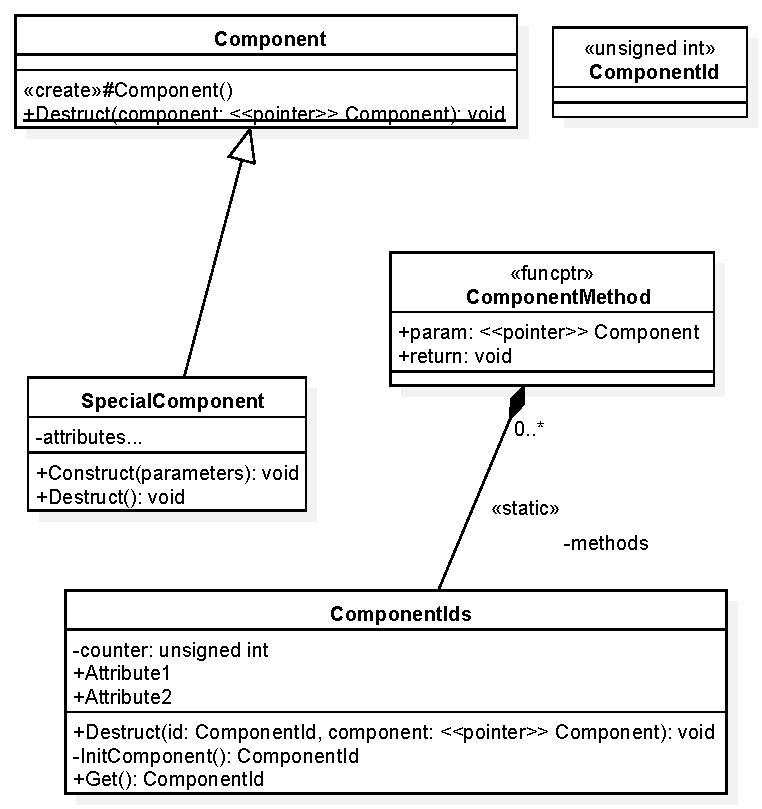
\includegraphics[width=\textwidth]{03unserprogramm/Engine/SpecialComponent.pdf}
		Die Klasse SpecialComponent ist eine Beispiel-Klasse für einen benutzererstellten Komponenten. Hierbei ist attributes für tatsächliche Variablen auszutauschen und parameters für die Parameter, die der Komponent benötigt um initialisiert zu werden. Es können gegebenenfalls auch mehrere Überladungen der Construct-Methode erstellt werden.
		\caption{Klassendiagramm der Component-Klassen}\label{ClassDiagramComponents}
	\end{center}
\end{figure}

Möchte man eine neue Komponente erstellen, so muss man eine Klasse erstellen, die von der Klasse Component erbt. Die Component-Klasse ist eine leere Klasse und dient nur dazu, verschiedene Komponenten auf eine allgemeine Weise zu speichern. 
\todo[inline]{KOMISCHER SATZ: START}
Wenn eine neue Komponente erstellt wird nicht unbedingt der Konstruktor aufgerufen wird, wenn ein alter Komponent wieder verwendet werden kann, muss jede Klasse, die von Component erbt die Methode Construct mit beliebigen Parametern enthalten, sowie die Methode Destruct ohne Parameter. 
\todo[inline]{KOMISCHER SATZ: ENDE}
Da Vererbung in diesem Fall einen großen Geschwindigkeitsverlust bewirken würde, muss die \textit{Construct}-Methode mit Hilfe von Templates aufgerufen werden. Bei der \textit{Destruct}-Methode ist dies leider nicht so einfach möglich, da der Datentyp zum Zeitpunkt der Zerstörung nicht mehr bekannt ist muss ein Funktions-Pointer für jeden Komponenten-Typ gespeichert werden. Dieser zeigt auf eine Funktion, welche einen \textit{Component}-Pointer erst zu dem spezifischen Komponenten-Pointer casted und dann die Destruct-Methode aufruft. Diese Funktion ist eine statische Template-Methode in der Component-Klasse. Mit dem Template-Parameter ist es möglich diese Methode für verschiedene Komponenten zu verwenden. Der Pointer wird in einem Objekt der Klasse \textit{EntityIds} gespeichert und kann verwendet werden, indem die statische Methode \textit{Destruct} aufgerufen wird, der sowohl die Komponente, als auch die ID übergeben wird. 
Er wird beim erstmaligen aufrufen der Methode Get() für jeden Komponent-Typ mit der Methode InitComponent() erstellt. Diese Klassen sind in \cref{ClassDiagramComponents} dargestellt.

Ein Manager ist eine Klasse, die von der Basisklasse \textit{Manager} erbt. 
\todo[inline]{Erklärung des Managers}

\subsection{Tasten-Eingabe System}
Natürlich benötigt ein Spiel auch ein sicheres Eingabe-System, welches sowohl die Position der Maus ermittelt, aber auch die Abfrage jeder einzelnen Taste auf der Tastatur regelt. 
Dafür wurde in der FM3D-Engine eine eigene Klasse implementiert, welche sich um dies kümmert.
Um den Nutzer der FM3D-Engine davor zu bewahren nicht jeden einzelnen ASCII-Code jeder Taste auf der Tastatur nachzuschlagen, sind alle Tasten in Form von Makros definiert. 
In dem Namespace FM3D befindet sich die Klasse Inputsystem. Diese Klasse besitzt eine rekursive Instanz, mit welcher man das Inputsystem ansprechen kann. 
Die Klasse beinhaltet außerdem die Enumeration \textit{KEYCLICK}, welches den aktuellen Stand der Maustasten beschreibt. Diese können entweder gedrückt, nicht gedrückt oder losgelassen werden und sind in dieser Enumeration definiert.
Eine Struktur \textit{MOUSE} enthält die Enumeration \textit{KEYCLICK} und einen zweidimensionalen Vektor des Typen \textit{Float}, welcher die zweidimensionale Position im Fenster angibt, an welcher eine Taste der Maus gedrückt wurde.
Diese Struktur wird im Inputsystem als ein vier-Felder Array verwendet, welches jede Taste einer durchschnittlichen Maus beschreibt. Diese sind die linke, die rechte und die mittlere Maustaste. 
Zudem besitzt das \textit{Inputsystem} einen Vektor \textit{lastposinst}, welcher ununterbrochen die Position der Maus ermittelt. Dies ist in den Spielen erforderlich in denen die Maus ununterbrochen die Kamera steuert.

Für die Tastenabfrage wurde zunächst ein Integer Wert verwendet, in welchen der aktuell gedrückte ASCII-Code gespeichert wurde. Dies hat aber den Nachteil, dass nur eine Taste gedrückt sein bzw. abgefragt werden kann. Möchte man nun zum Beispiel einen Spiele-Charakter schräg durch einen Raum durch gedrückte Links- \textbf{und} Rechts-Taste bewegen, so wäre das mit dieser Möglichkeit nicht möglich. Deswegen beschreibt nun ein 121-Felder Array aus booleschen Werten die komplette Tastatur. Jede Feldnummer ist äquivalent zu dem zugeordneten ASCII-Code der Taste. Die Felder [1] bis [4] beschreiben die Maustasten. Einige Felder des Arrays sind nicht von einem ASCII Code auf der Tastatur \textit{belegt} und sind somit "`\textit{frei}"'. Dies hat den Vorteil, dass später simpel weitere Eingabegeräte in das Inputsystem eingebunden werden können.

Die Klasse besitzt Methoden, welche in der Klasse Win32Window.h (Siehe Doxygen Dokumentation), die ein GUI-Fenster abbildet, um die verschiedenen Werte der Arrays und des Vektors zu setzen.
Zudem besitzt die Klasse Methoden, die diese Werte zurück geben. (Für die Verwendung dieser Klasse siehe \cref{inputsystemver})